

\documentclass[a4paper,14pt ]{article} % можно использовать кегель 8-12, 14, 17 и 20 пунктов
\DeclareMathSizes{14}{14}{14}{14}
\usepackage{extsizes}
\usepackage{graphicx}
\graphicspath{{/home/misha/VUZ/TOE/MATLAB}}
\usepackage[russian]{babel} % задаёт русский как основной язык текста
\usepackage[T2A]{fontenc} % задаёт кириллическую кодировку шрифта
\usepackage{cmap} % обеспечивает нормальное копирование и поиск русского текста в pdf 
\usepackage[utf8]{inputenc} % определяет юникодную кодировку самого .tex-файла
\setcounter{secnumdepth}{0}
\usepackage{geometry} % задаёт поля 
\geometry{left=3cm} % левое — 3 см
\geometry{right= 1.5cm} % правое — 1,5 см
\geometry{top=2cm} % верхнее — 2 см
\geometry{bottom=2cm} % нижнее — 2 см
\usepackage{setspace} \onehalfspacing % задаёт «полуторный» межстрочный интервал 
\usepackage{indentfirst} % автоматически добавляет отступ в каждый новый абзац
\usepackage{amsmath,amsfonts,amssymb,amsthm,mathtools,mathtext, physics}
\usepackage{float}
\usepackage{array}
\usepackage{tabularx}
\usepackage{titlesec}
\titleformat{\section}{\centering\normalfont\bfseries}{\thesection}{1em}{}
\setlength\parindent{1.25cm}
\begin{document} 
\begin{titlepage}
    \begin{center}
        {\bf  МИНОБРНАУКИ РОССИИ\\
        САНКТ-ПЕТЕРБУРГСКИЙ ГОСУДАРСТВЕННЫЙ\\
        ЭЛЕКТРОТЕХНИЧЕСКИЙ УНИВЕРСТИТЕТ\\
        <<ЛЭТИ>> ИМ. В. И. УЛЬЯНОВА (ЛЕНИНА)\\
    
        }
    \end{center}
    \vfill
        {
        \begin{center}
            КУРСОВАЯ РАБОТА\\
            по дисциплине <<Теоретические основы электротехники>>\\
            Тема: <<исследование прохождения сигналов через линейную активную электрическую цепь>>\\
        \end{center}
        }
        \
    \vfill
        {\noindent\parbox{4cm}{Студент гр. 3114}  \hfill \parbox{3cm}{\rule{3cm}{0.15mm}} \hfill \parbox{4cm}{\raggedleft Злобин М. А.}\\}
        \parbox{4cm}{Преподаватель} \hfill \parbox{3cm}{\rule{3cm}{0.15mm}} \hfill \parbox{4cm}{\raggedleft Завьялов А. Е.} \\ 
        \center Санкт-Петербург
        
        2024
\end{titlepage}
\begin{center}
    {\bf АННОТАЦИЯ} 
\end{center}
    

    {
    Линейные электрические цепи играют ключевую роль в усилении и обработке сигналов, 
    проходящих через них. Для анализа таких цепей применяются методы преобразования Лапласа, 
    разложения в ряды Фурье и спектрального анализа. Изучение линейных цепей и сигналов, 
    которые через них проходят, позволяет предсказывать поведение схем при воздействии на них периодических сигналов.
    }
\begin{center}
    {\bf SUMMARY}
\end{center}


Linear electrical circuits are essential for amplifying and\\ processing the signals passing through them. 
Methods such as Laplace transform, Fourier series decomposition, and spectrum analysis are used to analyze these circuits. 
Studying linear circuits and the signals that pass through them allows for predicting the behavior of the circuit when subjected to certain periodic signals.
\newpage
\tableofcontents
\newpage
\section{ВВЕДЕНИЕ}
Цель курсовой работы – практическое освоение методов анализа искажений электрических сигналов, проходящих через линейные активные   RC~– цепи, а также рассмотрение вопросов проектирования активных RC – цепей по заданным передаточным функциям. 
В курсовой работе требуется выполнить следующие пункты: 
    \begin{enumerate}
        \item Найти по заданной передаточной функции реакцию активной RC-цепи при воздействии одиночного импульса; 
        \item Рассчитать переходную и импульсную характеристики активной цепи;  
        \item Найти спектральные характеристики аналогового входного сигнала и частотные характеристики цепи;  
        \item Вычислить 	установившуюся 	реакцию 	цепи 	при 	воздействии 
        периодической последовательности импульсов;  
        \item Рассчитать параметры элементов активной цепи по заданной передаточной функции.
    \end{enumerate}
    \newpage
    \section{Нормирование параметров и переменных цепи}
    Произведем нормировку переменных и параметров электрической \\ цепи:
    \begin{table*}[h!]
        \centering
        \begin{tabularx}{\linewidth} { |>{\raggedright\arraybackslash}X | X | X |}
            \hline
           $ t_\text{и} = 2 \, \text{мс} $ & $ U_\text{m} = 3 \, \text{В} $ & $T = 2t_\text{и} = 4 \, \text{мс}$ \\ \hline
           $ t_\text{б} = 1 \, \text{мс} $ & $ U_\text{б} = 1 \, \text{В} $ & $T_\text{б} = 1 \, \text{мс} $ \\ \hline 
           $ t^*_\text{и} = \frac{t_\text{и}}{t_\text{б}} $ &  
            $ U^*_\text{б} = \frac{U_\text{m}}{U_\text{б}} $ &
            $ T^* = \frac{T }{T_\text{б}} $ \\ \hline
            $ R_\text{б} = 10^{-5} \,\text{Ом}$ & $C_\text{б} = \frac{ t_\text{б}}{R_\text{б}} $ & $C^* = \frac{C}{C_\text{б}} $ \\
            \hline
        \end{tabularx}
        \caption{Нормирование параметров цепи}
        \label{table:1}
    \end{table*}

    \it{Замечание}\normalfont: все дальнейшие расчеты в курсовой работе выполняются с нормированными параметрами, поэтому для упрощения всех дальнейших записей знак (*) будет опускаться.
    \section{Записать передаточную фикцию актовой RC-цепи с заданными коэффициентами. Рассчитать нули и полюсы заданной передаточной функции активной цепи. Изобразить координаты вычисленных нулей и полюсов на комплексной плоскости; найти приблизительную длительность свободного процесса в активной цепи по значению вещественной части полюсов}
    Передаточная функция $H_U(S) = \frac{U_1(S)}{U_2(S)} = \frac{a_2S^2 + a_1S + a_0}{S^2 + b_1S+b_0}$\\
    $a_1 = 0; a_2 = 0; a_0 = 5.52; b_1 = 2.2; b_0 = 4.4$;
    $H_U(S) = \frac{5.52}{S^2 + 2.2S+ 4.4}$;
    
    Найдем полюсы передаточной функции: 
        $S_1 = -1.1 + 1.77j; S_2 = -1.1 - 1.77j$.

    Нулей у передаточной функции нет.


    Изобразим полюсы на комплексной плоскости (рис. \ref{fig:1}):
    \begin{figure}[H]
        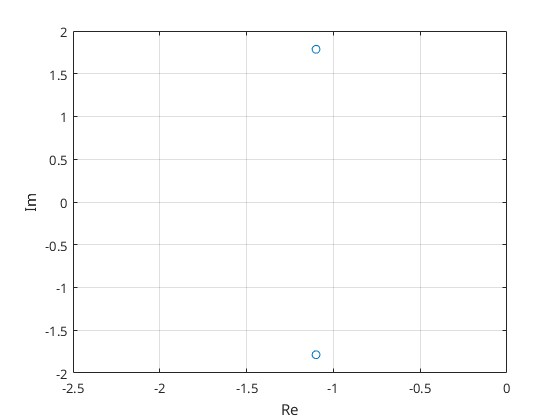
\includegraphics[width=0.65\textwidth]{poluses}
        \centering
        \caption{Полюсы передаточной функции}
        \label{fig:1}
    \end{figure} 
    \section{Найти изображение входного одиночного импульса воздействия и вычислить реакцию активной RC-цепи операторным методом; построить график реакции; приближенно оценить время затухания переходных процессов в цепи.}
    Найдем изображение импульса типа меандр (Рис. \ref{fig:2} )
    \begin{figure}[H]
        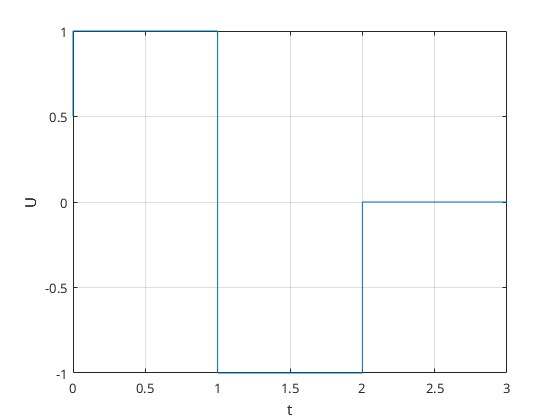
\includegraphics[width=0.65\textwidth]{imp}
        \centering
        \caption{Импульс меандр}
        \label{fig:2}
    \end{figure}
    С учетом данных таблицы \ref{table:1}, временная функция этого импульса будет выглядеть так:
    \begin{equation}
        u_1(t) = 3\delta (t) - 6\delta(t-1) + 3\delta(t-2),
    \end{equation}


    тогда изображение этого импульса:
    \begin{equation}
        U_1(S) = \frac{1}{S}\left(3e^{-2S} - 6e^{-S} + 3\right). 
    \end{equation}

    Расчитаем реакцию цепи операторным методом:
    \begin{multline}
        U_2(S) = H(S)\cdot U_1(S) =  \frac{5.52}{S^2 + 2.2S+ 4.4}
        \cdot \frac{1}{S}\left(3e^{-2S} - 6e^{-S} + 3\right) = \\
        = \frac{5.52\cdot3}{S(S^2 + 2.2S+ 4.4)}\cdot e^{-2S} -
        \frac{5.52\cdot6}{S(S^2 + 2.2S+ 4.4)}\cdot e^{-S} + \\
        + \frac{5.52\cdot3}{S(S^2 + 2.2S+ 4.4)}.
    \end{multline}
    После разложения на простейшие и перехода {\it t}-область:
    \begin{multline}
        u_2(t) = 33.12\delta_1(1.0t - 1.0)
        (0.23e^{1.1 - 1.1t}(\cos(1.79t - 1.79) + \\
        + 0.62\sin(1.79t - 1.79)) - 0.23) - 
        3.76e^{-1.1t}(\cos(1.79t) + \\
        + 0.62\sin(1.79t)) - 16.56\delta_1(t - 2)(0.23e^{2.2 - 1.1t}
        (\cos(1.79t - 3.57) + \\
        + 0.62\sin(1.79t - 3.57)) - 
        0.23) + 3.76.
    \end{multline}
    Построим график реакции:
    \begin{figure}[H]
        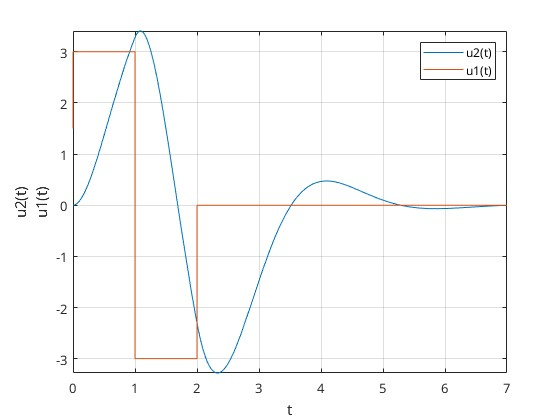
\includegraphics[width=0.8\textwidth]{react}.
        \centering
        \caption{график реакции вместе с графиком воздействия}
    \end{figure}
    \section{Вычислить переходную и 
    импульсную характеристики активной цепи по
     заданной передаточной функции; построить их графики.}
    Вычислим переходную характеристику активной цепи:
    \begin{multline}
        H_1(S) = \frac{H(S)}{S}= \frac{5.52}{S(S^2 + 2.2S+ 4.4)} = 
        -\frac{0.63 + j0.39}{S+1.1 + j1.79} - \\ - \frac{0.63 - j0.39}{S + 1.1 - j1.79} + \frac{1.26}{S}.
    \end{multline}
    \begin{equation}
        h_1(t) = 1.26 - 1.26e^{-1.1t}(\cos(1.79t) + 0.62\sin(1.79t)).
    \end{equation}
    Построим график переходной характеристики:
    \begin{figure}[H]
        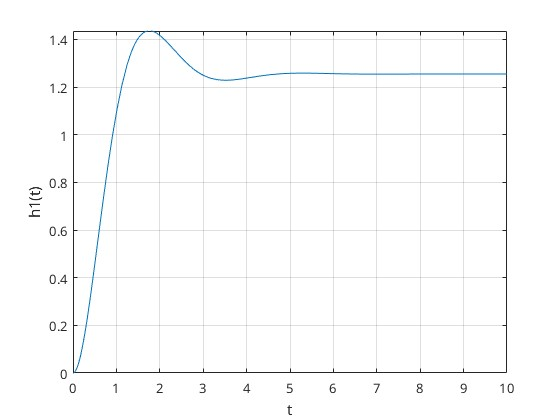
\includegraphics[width=0.8\textwidth]{h1}
        \centering
        \caption{Переходная характеристика}
    \end{figure}
    Вычислим импульсную характеристику активной цепи:
    \begin{multline}
        H(S) = \frac{5.52}{(S^2 + 2.2S+ 4.4)} = \frac{-1.54j}{S + 1.1 - j1.79} + \\ 
        + \frac{1.54j}{S - 1.1 + j1.79}.
    \end{multline}
    \begin{equation}
        h(t) = 3.09e^{-1.1t}\sin(1.79t).
    \end{equation}
    Построим график импульсной характеристики:
    \begin{figure}[H]
        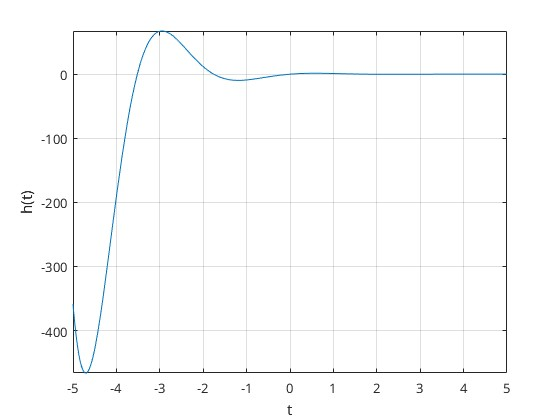
\includegraphics[width=0.8\textwidth]{h}
        \centering
        \caption{Импульсная характеристика}
    \end{figure}
    \section{Определить амплитудный и фазовый спектры входного одиночного импульса и построить их графики.}
    Входной одиночный импульс-меандр представлен на рисунке \ref{fig:1}.
    Определим амплитудный и фазовый спектры:
    \begin{multline}
        U_1(jw) = U_1(S)|_{jw} = \frac{1}{jw}\left(3e^{-2jw} - 6e^{-jw} + 3\right) = \\ 
         = \frac{3}{jw}e^{-jw}(e^{-jw} - 2 + e^{jw}) = 
         \frac{3}{jw}e^{-jw}\left(e^{-\frac{1}{2}jw} - e^{\frac12jw}\right)^2 = \\
         = j\frac{12}{w}e^{-jw}\sin^2\left(\frac12w\right).
    \end{multline} 
    \begin{equation}
        A(w) = \left| U_1(jw)\right| = 
        \frac{|j6e^{jw}\sin^2\left(\frac12w\right)
        |}{w}. 
    \end{equation}
    \begin{multline*}
        A(w)|_{w=0}=\lim\limits_{w \to 0}
        \frac{|j12e^{jw}\sin^2\left(\frac12w\right)
        |}{w} = \lim\limits_{w \to 0}
        \frac{\left(12\sin^2\left(\frac12w\right)\right)'
        }{1} = \\
        = \lim\limits_{w \to 0}12\left(2sin\left(\frac12w\right)
        \frac12\cos\left(\frac12w\right)\right) = 0.
    \end{multline*}
    \indent Значение спектрально плотности в нуле равно площади импульса, 
    что выполняется, т. к. алгебраическая площадь меандра равна нулю,\
    что видно из рис. \ref{fig:1}
    \begin{multline}
        \Phi(w) = \arg\left(
            j\frac{12}{w}e^{-jw}\sin^2\left(\frac12w\right)
            \right) = \\ = \arg\left(je^{-jw}\sin^2\left(\frac12w\right)\right) = 
            \frac{\pi}2 - w.
    \end{multline}
    \indent Построим графики амплитудной и фазовой спектральной плотности:
    \begin{figure}[H]
        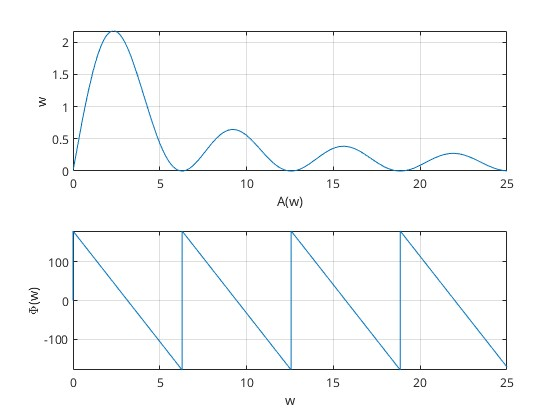
\includegraphics[width=0.8\textwidth]{awpw}
        \centering
        \caption{амплитудный и фазовый спектры одиночного импульса-меандра}
        \label{fig:6}
    \end{figure}
    \newpage
    \section{Рассчитать амплитудно-частотную (АЧХ) и фазочастотную (ФЧХ) характеристики активной цепи; построить графики АЧХ- и ФЧХ-цепи, а также график амплитудно-фазовой характеристики; определить полосу пропускания цепи и оценить время запаздывания сигналов, спектр которых попадает в полосу пропускания.}
    Рассчитаем АЧХ как $|H_U(j\omega)|$, $H_U(j\omega) =  
    H_U(S) = \frac{5.52}{(j\omega)^2 + 2.2j\omega+ 4.4}$;
    \begin{equation}
        A(\omega) = \frac{5.52}{\sqrt{(2.2j\omega)^2 + (4.4 - \omega^2)}}.
    \end{equation}

    Рассчитаем ФЧХ как $arg(H(j\omega))$:
    \begin{equation}
        \Phi(\omega) = 0 - arg(2.2j\omega + (4.4 - \omega^2)).
    \end{equation} 
    
    Построим графики:
    \begin{figure}[H]
        \centering
        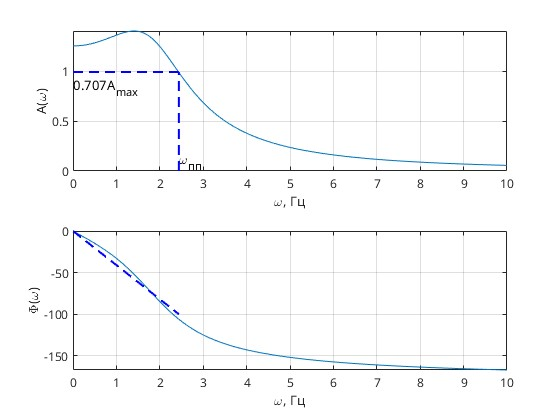
\includegraphics[width=0.75\linewidth]{ampl_phase}
        \caption{AЧХ и АФХ активной цепи}
    \end{figure}
    
    Граница полосы пропускания цепи $\omega_\text{пп} = 2.44$ Гц ($A_{max} = 1.4048$),
    время задержки $t_\text{з} = 0.71$.
    
    Рассчитаем АФХ как $H_U(j\omega) = A(\omega)^{-\Phi(\omega)j}$:
    \begin{equation}
        H(j\omega) = \frac{5.52}{\sqrt{(2.2j\omega)^2 + (4.4 - \omega^2)}}e^{-j(0 - arg(2.2j\omega + (4.4 - \omega^2)))}.
    \end{equation}
    Построим график:
    \begin{figure}[H]
        \centering
        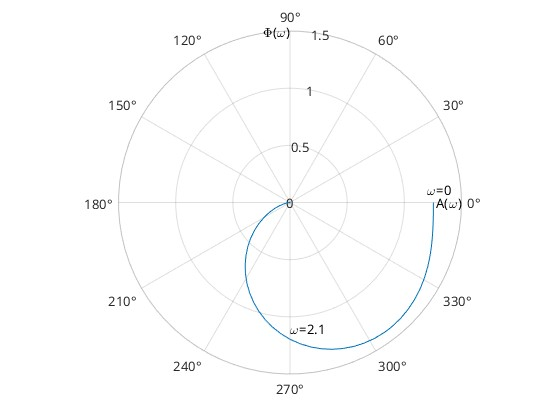
\includegraphics[width=0.75\linewidth]{polarplot}
        \caption{AФХ активной цепи.}
    \end{figure}
    \section{Определить амплитудный и фазовый спектры периодического 
    входного сигнала;
     ограничиться 10 гармониками разложения сигнала в ряд Фурье; 
     построить графики исходного входного периодического сигнала и сигнала, представленного рядом Фурье 
    (изобразить отдельно 3 первые составляющие ряда).}
    Рассмотрим периодический сигнал формы меандра (Рис. \ref{fig:2}) c параметрами, 
    приведенными в таблице \ref{table:1}. $t_\text{и} = 4, \omega_1 = 2\pi/t_\text{и} = 
    1.57$ Гц.
    Амплитудный и фазовый спектры периодическго сигнала связаны со спектральной плостностью
    апериодического импульса соотношениям
    \begin{equation}
        \begin{cases}
            A_0 = \frac{1}{T}A(0);\\
        A_k = \frac{2}{T}A(\omega_k);\\
        \Phi_k = \Phi(\omega_k),
        \end{cases}
    U_1 = A_0 + \sum_{k=1}^{10}A_{k}\cos(\omega t + \Phi_{2k}).
    \end{equation}

    где $\omega_k = \omega_1 k$. Составим таблицу расчетов для фазы и амплитудный
    первых 10 гармоник:
    \begin{table*}[h!]
        \centering
        \begin{tabularx}{\linewidth} { | X | X | X | X | X | X | X | X | X | X | X | X |}
            \hline
            k & 1 & 2 & 3 & 4 & 5 & 6 & 7 & 8 & 9 & 10\\
            \hline
            $A_k$ & $12/\pi$ & $12/\pi$ & $4/\pi$ &0  & $12/5\pi$ & $4/\pi$& 
            $12/7\pi$ & 0 & $4/3\pi$ & $12/5\pi$ \\
            \hline
            $\Phi_k$ & 0 & $ -\pi/2 $ & $\pi$ & 0 & 0 & $-\pi/2$ & $\pi$ & 0 & 0 & $-\pi/2$\\
            \hline
        \end{tabularx}
        \caption{Расчеты амлитуды и фазы периодического сигнала}
        \label{table:2}
    \end{table*}
    
    Построим графики амплитудного и фазового спектра:
    \begin{figure}[H]
        \centering
        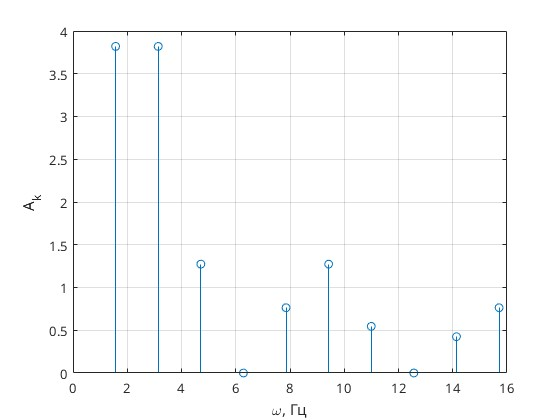
\includegraphics[width=0.75\linewidth]{amplitude}
        \caption{Амплитудный спектр периодическго сигнала}
        \label{fig:7}
    \end{figure}
    \begin{figure}[H]
        \centering
        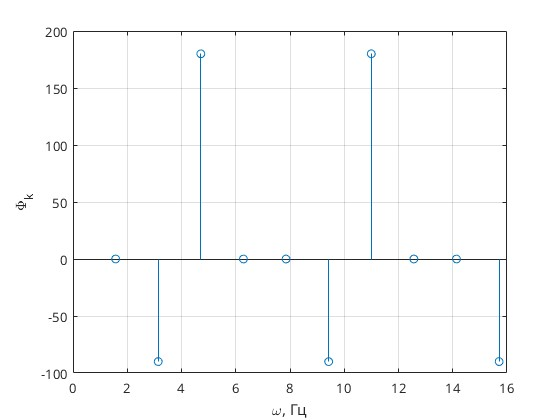
\includegraphics[width=0.75\linewidth]{phase}
        \caption{Фазовый спектр периодическго сигнала}
        \label{fig:8}
    \end{figure}
    Изобразим первые три ненулевые составляющие ряда Фурье:
    \begin{figure}[H]
        \centering
        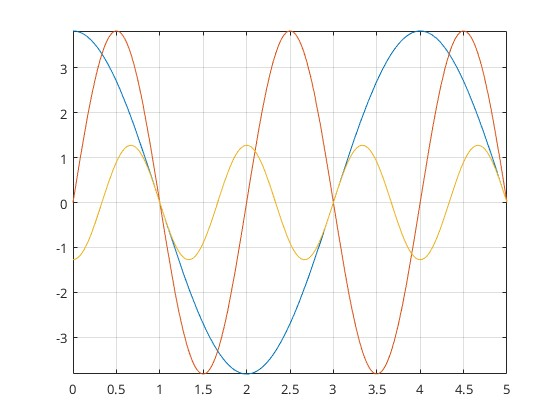
\includegraphics[width=0.75\linewidth]{3garm}
        \caption{Три первые ненулевые гармоники ряда Фурье}
        \label{fig:8}
    \end{figure}
\section{Произвести приближенный расчет реакции цепи по спектру при периодическом воздействии; построить график реакции; оценить искажения передачи сигналов при прохождении через исследуемую активную цепь сравнением ширины спектра воздействия и полосы пропускания цепи.}
Аплитудный и фазовый спектр периодической реакции определяются следующими
выражениями:
\begin{equation}
    \begin{cases}
        A_{2k} = A_k A(k\omega);\\
        \Phi_{2k} = \Phi_k \Phi(k\omega);
    \end{cases}
    U_2 = \sum_{k=1}^{10}A_{2k}\cos(k\omega t + \Phi_{2k}).
\end{equation}
 Составим таблицу расчетов для фазы и амплитуды первых 10 гармоник реакции:

    \begin{table*}[h!]
        \centering
        \begin{tabularx}{\linewidth} { | X | X | X | X | X | X | X | X | X | X | X | X |}
            \hline
            k & 1 & 2 & 3 & 4 & 5 & 6 & 7 & 8 & 9 & 10\\
            \hline
            $A_2k$ & $2.66$ & $1.19$ & $0.17$ &0  & $0.035$ & $0.04$& 
            $0.01$ & 0 & $0.01$ & $0.008$ \\
            \hline
            $\Phi_2k$ & 0 & $ -61 $ & $-218$ & 30 & -158 & $-163$ & $-256$ & 12 & -169 & $-170$\\
            \hline
        \end{tabularx}
        \caption{Расчеты амлитуды и фазы периодической реакции}
        \label{table:3}

    \end{table*}
    Построим график реакции цепи:
    \begin{figure}[H]
        \centering
        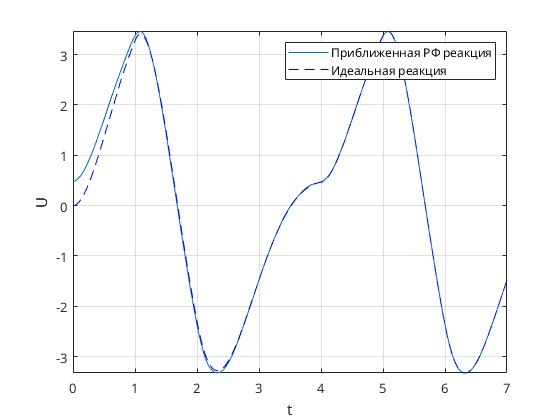
\includegraphics[width=0.75\linewidth]{reactRF}
        \caption{График реакции}
        \label{fig:10}
    \end{figure}
   Для оценки искажения сигнала рассмотрим ширину полосы пропускания АЧХ и 
   ширину амплитудного спектра при периодическом воздействии по двум критериям:
   \begin{itemize}
    \item Граница пп $\omega_\text{пп} = 2.44$ Гц.
    \item Критерий 10\%: $\omega_\text{10\%} = 8\pi$.
    \item Критерий первого лепестка: $\omega_\text{} = 2\pi$ Гц.
   \end{itemize}

   По обоим критериям полоса пропускания меньше ширины спектра входного сигнала, поэтому 
   форма сигнала после прохождения через цепь в значительной степени изменена. 
\section{Вычислить параметры активной RC-цепи второго порядка, используя заданную передаточную функцию}
   Параметры элемента активного звена будем вычислять по заданным коэффициентами ПФ:
   $ H(S) = \frac{5.52}{(S^2 + 2.2S+ 4.4)} $.
   \\
   \\
   \\
   \\
   \\
   \\
   \\

   Перед
составлением системы алгебраических уравнений с использованием метода
узловых напряжений предварительно выполним в схеме преобразование
входного источника напряжения $\dot{U_1}$ с последовательно соединенным напряжением
$R_2$ в источник тока $\dot{U_1}G_2$.
Составленная с помощью МУН система уравнений выглядит следующим образом:
\begin{equation}
    \begin{cases}
        (Z_3 + G_2 + G_4 + G_7)\dot{U_1^y} - G_4\dot{U_2^y} - G_7\dot{U_3^y} = G_2\dot{U_1};\\
        -G_4\dot{U_1^y} +(Z_5 + G_4)\dot{U_2^y} = 0.\\
        \dot{U_3^y} = kU_2^y;
    \end{cases}
\end{equation} 

Для упрощения анализа активной
RC-цепи можно принять равенство параметров пассивных элементов:
$R_2 = R_4 = R_7 = R$ и $Z_3 = Z_5 = Z = sC$.
Получим:
\begin{equation}
    \begin{cases}
        (Z_c + 3G)\dot{U_1^y} - G(1+k)\dot{U_2^y} = G\dot{U_1};\\
        -G\dot{U_1^y} +(sC + G)\dot{U_2^y} = 0.\\
        \dot{U_3^y} = kU_2^y;
    \end{cases}
\end{equation}
\begin{equation}
    H(s) = \frac{U_2(s)}{U_2(s)} = \frac{\dot{U_3^y}}{U_1(s)} = 
    \frac{\frac{k}{R_*^2C_*^2}}{s^2 + s\left(\frac{3}{R_*C_*}\right) + \frac{1+k}{R_*^2C_*^2}},
\end{equation}

где $R_*, \, C_*$ -- нормированные параметры элементов цепи.
Произведя сравнение коэффициентов полиномов знаменателей обеих
дробей выражения, составим два компонентных уравнения с нормиро-
ванными параметрами элементов:
\begin{equation}
    \begin{cases}
        \frac{3}{R_*C_*} = 2.2;\\
        \frac{1+k}{(R_*C_*)^2} = 4.4.
    \end{cases}
\end{equation}

Примем в качестве известного параметра емкость $C_* = 1$. тогда
сопротивление $R_* = 1.34$. Коэффициент усиления усилителя $k = 2(R_*C_*)^2 = 3.59$.

Используя известные базисные параметры элементов $R_\text{б} = 100$ кОм, $C_\text{б} = 10^{-8}$ Ф 
получаем $R_2 = R_4 = R_7 = 134$ кОм, $C_3 = C_5 = 0.01$ мкФ.
\section{Вывод}
В ходе работы были выполнены:
\begin{itemize}
    \item нормировка параметров и переменных цепи, необходимые для удобства расчётов; 
    \item расчёты нулей и полюсов функции передачи, что необходимо для того, чтобы убедиться в устойчивости (способность цепи возвращаться в исходный установившийся режим) системы, так же был определён тип фильтра(ФНЧ); 
    \item нахождение изображения водного одиночного импульса воздействия и вычисление реакции цепи, а также построен её график, данные полученные на данном этапе использовались в дальнейших расчётах;
    \item нахождение операторным методом импульсной и переходной характеристик цепи, где импульсная характеристика – это демонстрация реакции цепи на единственное воздействие вида единичной импульсной функции, переходная характеристика – это демонстрация реакции цепи на единственное воздействие вида единичной ступенчатой функции;
    \item нахождение амплитудного и фазового спектров входного одиночного импульса;
    \item нарождение АЧХ, ФЧХ и АФХ, построение их графиков, определение полосы пропускания цепи и времени задержки сигнала;
    \item нахождение амплитудного и фазового спектров периодического водного сигнала, разложение пародического воздействия в ряд Фурье;
    \item расчёт реакции цепи по спектру при периодическом воздействии, сделан вывод о прохождении сигнала через заданную цепь;
    \item вычисление параметров активной RC – цепи, при помощи заданной функции передачи.
\end{itemize}
\newpage
\section{СПИСОК ИСПОЛЬЗОВАННЫХ ИСТОЧНИКОВ}
\begin{enumerate}
    \item Бычков Ю.А., Золотницкий В.М., Чернышев Э.П., Белянин А.Н. Основы теоретической электротехники: Учебное пособие. СПБ.: Изд-во “Лань”, 2008.  592 с.: ил. – (Учебники для вузов. Специальная литература). 
    \item Бычков Ю.А., Соловьева Е.Б., Чернышев Э.П. Курсовое проектирование по теоретической электротехниче: учеб. пособие в 2 ч. Ч. 1. СПб.: Изд-во СПбГЭТУ "ЛЭТИ", 2017. 109 с. 
    \item Иншаков Ю. М., Портной М. С. Исследование прохождения сигналов через линейную активную цепь: учеб.-метод. пособие. СПб.: Изд-во СПбГЭТУ "ЛЭТИ", 2024. 48 с. 
\end{enumerate}
\end{document}

